% !TEX encoding = UTF-8
% !TEX TS-program = pdflatex
% !TEX root = ../tesi.tex

%**************************************************************
\chapter{Comparison between the languages for Pulumi and the advantages of Scala}
\label{cap:comparisons}
%**************************************************************

\intro{Here all the advantages and disadvantages detected while using Typecript and Scala for our case study will be presented.}\\

%**************************************************************
\section{Code readability in Typescript vs in Scala}

\subsection{Readability in Typescript}
Typescript is less verbose than many other programming languages.
In the implementation we can appreciate how the passing of the builders methods' parameters have been achieved in a concise way using the JSON format.
This is fitting very well in a declarative approach and is very readable and intuitive, but some lacks of the language caused the code to lose readability and conciseness.

\subsubsection{Less readable code with pulumi.all and .apply}
\label{sssec:ts-subnets-comparison}
Lets consider once again the Typescript version of the function that is responsible for creating the subnets across the various availability zones:
\begin{center}
  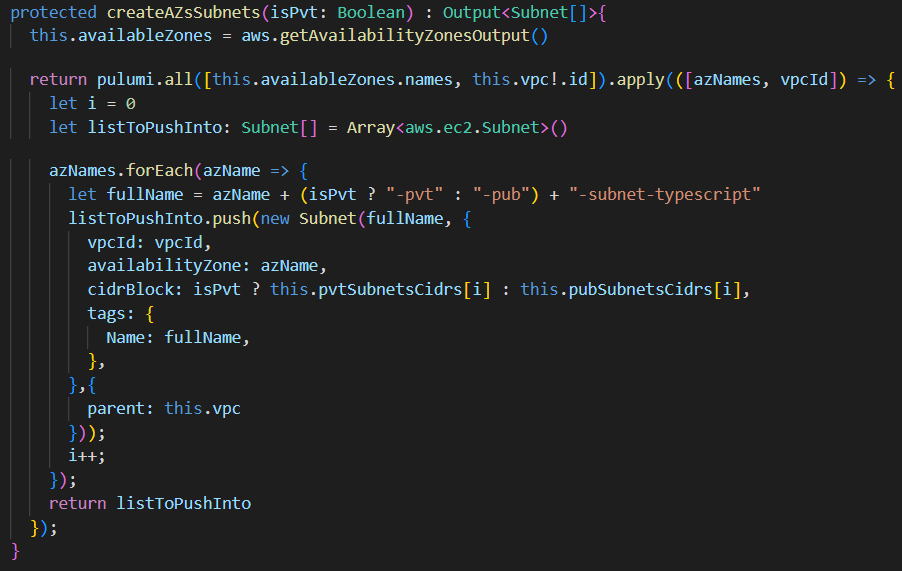
\includegraphics[width=1.0\columnwidth]{comparisons/ts_create_subnets} 
  \captionof{figure}{Typescript subnets creation}
\end{center}\mbox{}\\
When talking about readability, the \texttt{pulumi.all} and the \texttt{apply} functions are quite cryptic.
It takes us a little time to understand what are the return types of the \texttt{pulumi.all} and of the \texttt{apply} functions.
I remind here that the types of these two functions are fully explained in the \hyperref[par:ts-lambda]{The apply's lambda} paragraph.\\
We'll make furthers considerations on this function in the \hyperref[sssec:readability-for-yield]{Readability of the Scala's for yield vs pulumi.all and .apply} paragraph.

\subsection{Readability in Scala}
Also in Scala, thanks to the syntactic sugar used, we achieved a surprisingly readable code while defining the resources to be created on our Pulumi stack.

\subsubsection{Function currying}
The currying of Scala used to define our \textit{sugarized} functions granted us the possibility to declare the resources with this syntax:
\begin{verbatim}
  val resourceName = sugarizedResourceConstructor("res-name") {
    firstParameter(...)
    secondParameter(...)
    ...
  }
\end{verbatim}\mbox{}\\
This code is really readable (it resembles to a function definition) and is perfectly fitting in a declarative approach since we can have a straight list of the parameters we want to set for our resource.\\

\subsubsection{Hidden builders}
Thanks to the \texttt{given} and \texttt{using} keywords, builders aren't manually instantiated and we don't require to explicitly say on which builder instance we are calling the builders' methods.
This is letting us have an even more lightweight code that is really just focusing on what we need to instantiate instead of the how we could instantiate it.
Let's consider the VPC creation in our Scala solution and how would it is it created instead in a Java solution.\\
Scala solution:
\begin{lstlisting}[numbers=left, numberstyle=\tiny, numbersep=-5pt, stepnumber=1]
  val myVpc = vpc("scala-main") {
    cidrBlock("10.136.0.0/24")
    tags("Name" -> "myVpcScala")
  }
\end{lstlisting}\mbox{}\\
Java solution:
\begin{lstlisting}[numbers=left, numberstyle=\tiny, numbersep=-5pt, stepnumber=1]
  protected Vpc vpc = new Vpc("my-vpc-java", VpcArgs.builder()
    .cidrBlock("10.136.0.0/24")
    .instanceTenancy("default")
    .tags(Map.of("Name", "myVpcJava"))
    .build(),
          CustomResourceOptions.builder()
                  .parent(this)
                  .build());
\end{lstlisting}\mbox{}\\
Even if our syntactic sugar is using the very same APIs used from the Java's solution, the readability and the conciseness are entirely on another level.

\subsubsection{Implicit conversion functions to get rid of Map and List constructors while passing a single value}
The implicit conversion functions presented in the \hyperref[sssec:implicit-converion-functions]{Implicit conversion functions} paragraph let us get rid of the constructor of the Map and of the List if we're interested in passing a single value.\\
It is common, while declaring a new resource, to pass a single parameter to a builder's method that is actually expecting a list or a map of parameters.
In such cases the following syntax could be annoying:
\begin{center}
  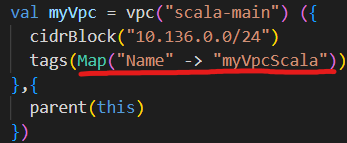
\includegraphics[width=0.7\columnwidth]{comparisons/explicit_map} 
  \captionof{figure}{Singleton map for a parameter}
\end{center}\mbox{}\\
%Tags expects a \texttt{Map[String, String]} value, but if we want to pass a single map element, we would appreaciate to get rid of the Map constructor and just write \texttt{"Name -> "myVpcScala"}.
But thanks to the implicit conversion functions the final result, as we have seen, is the desired one:
\begin{center}
  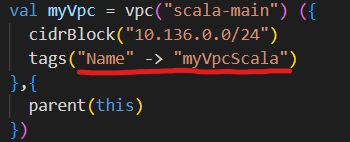
\includegraphics[width=0.7\columnwidth]{comparisons/implicit_map} 
  \captionof{figure}{Tuple for a parameter}
\end{center}\mbox{}\\
For a single parameter the difference of effort in explicitly writing the map constructor can be negligible, but when it comes to define many resources that use multiple methods that accept collections as input parameters, such a feature can really save us a lot of keystrokes, while keeping our code more readable and simple.

\subsubsection{Readability of the Scala's for yield vs pulumi.all and .apply}
\label{sssec:readability-for-yield}
Lets consider the function that creates the subnets.
With respect to the Typescript solution, the Scala one is more readable:
\begin{center}
  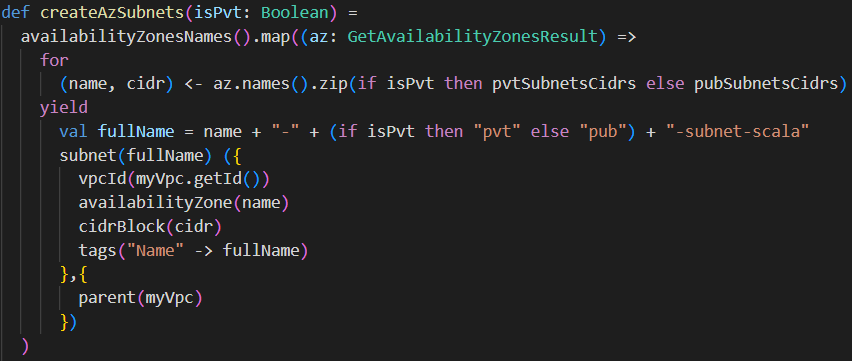
\includegraphics[width=1.0\columnwidth]{comparisons/scala_create_subnets} 
  \captionof{figure}{Scala subnets creation}
\end{center}\mbox{}\\
First, the \texttt{map} function is much more intuitive with respect to the \texttt{pulumi.all} and \texttt{apply} combination in the \hyperref[sssec:ts-subnets-comparison]{Typescript implementation}.
Moreover, the for comprehension used in the Scala version is a more elegant and concise solution.
In fact, the map function is doing the work of both the \texttt{pulumi.all} and \texttt{apply} functions, with much less code and in a much more readable way.\\
Furthermore, with Scala we're using the language feature of the for comprehension to automatically create a collection of the generated subnets and return them all together.\\
Differently, Typescript implementation requires us to explicitly insert the generated subnets in a variable as a side effect of the \texttt{foreach}.
Moreover, with Typescript, we also have to explicitly return the list at the end of the \texttt{apply}'s lambda.


\section{Expressiveness in Typescript vs in Scala}

\subsection{pulumi.all and .apply vs for comprehension and monads}

\subsubsection{Typescript compensate for its lack of expressiveness with the pulumi.all function}
In the \hyperref[sssec:pulumi-all]{pulumi.all} paragraph of the subnets creation section, we have seen how the concatenation of \texttt{apply} to the \texttt{pulumi.all} function let us create the subnets across the various availability zones.
Anyway, The process of wrapping two different \texttt{Ouptut} values in a single \texttt{Output} using the \texttt{pulumi.all} function, and then extract that newly created value form the \texttt{Output} context is verbose and complex.\\
Now, the \texttt{pulumi.all} function is effective but its existence is required to compensate for the lack of expressiveness of the Typescript language.

\subsubsection{Scala's expressiveness let us get rid of pulumi.all}
The functional nature of the Scala language let us get rid of the \texttt{pulumi.all} function thanks to the monad implementation for the \texttt{Output} type.
The \texttt{apply} function became the actual implementation of the \texttt{flatMap} function for the \texttt{Output[Monad]}.
The \texttt{map} function that we used in our function for the \hyperref[sssec:subnets-creation]{subnets creation} has been implemented only on the bases of the \texttt{flatMap} function.
So, we replaced the \texttt{pulumi.all} function with the \texttt{map} function offered by the \texttt{Monad[Output]}, and the \texttt{apply} function is now hidden behind the \texttt{map} implementation.\\
This achievement is perfectly depicting how the expressiveness of Scala permitted us to satisfy our need of applying functions on values contained inside a context (\texttt{Output} in our case), without resorting to an ad-hoc function created only for that specific purpose.
In fact, we would be able to implement a monad for any context type, while \texttt{pulumi.all} is working exclusively with the \texttt{Output} type.
Moreover, the \texttt{map} function is much more intuitive to an user rather than the \texttt{pulumi.all} and the explicit \texttt{apply} functions.

%On the other hand, when we have to combine two values of different \texttt{Output}s types in another value of another \texttt{Output} type, we must rely on the \texttt{pulumi.all} and \texttt{.apply} functions.
%In the \hyperref[sssec:pulumi-all]{pulumi.all} paragraph we have seen how such a function is used in the Typescript implementation to create the subnets in our availability zones.


%Now, if we want to use the \texttt{.apply} function to 
%since we have to pass through a pulumi.all to wrap the availability zones names \texttt{Output<String[]>} and the 


%\subsubsection{Poor tools to act on groups of Outputs}

%\section{Java solution observations}

%\subsection{Advantages of using Pulumi's Java APIs}

%\subsection{Disadvantages of using Pulumi's Java APIs}

%\subsubsection{Verbose code}

%\section{My Scala solution observations}

%\subsection{Advantages of using my Scala syntactic sugar}

%\subsubsection{Very concise code}

%\subsubsection{Very readable and elegant code}

%\subsubsection{More powerful constructs thanks to the for-comprehension and the monads to act on groups of Outputs}

%\subsection{Disadvantages of using my Scala syntactic sugar}

%\subsubsection{Partial solution, not all the corner cases have been considered}

%\section{Final thoughts on the Scala solution}